\section{这是怎样一种陈述？}\label{sec:1}

我将把几何朗兰兹对偶描述为谱定理（spectral theorem）的非阿贝尔对应物。为此，我们先回头重温谱定理。

\subsection{谱定理}\label{sec:1.1}

谱定理为希尔伯特空间 $\mathcal{H}$ 上的自伴算子（self-adjoint operator）$H$ 提供了一套谱分解理论。它为我们熟知的事实——实对称矩阵，或更一般地，复埃尔米特矩阵可以对角化——提供了普遍背景。该事实可以解释为：底层的希尔伯特空间 $\mathcal{H}\cong\C^{n}$ 分解为本征空间（eigenspace）的直和
\begin{equation}\label{eq:1.1}
\mathcal{H}\;\cong\;\bigoplus_{\lambda\in\R_{t}}\mathcal{H}_{\lambda}.
\end{equation}
我们可以把每个 $\mathcal{H}_{\lambda}$ 看作“生活在”相应的点 $\lambda\in\R_{t}$ 之上，于是对 $\R_{t}$ 的任意子集，都可把相应本征空间之和定义为与之对应的子空间。（这里 $\R_{t}$ 表示带坐标 $t$ 的一份 $\R$ 的拷贝，这是我们用来记本征值与谱测度之定义域的记号，即动量空间。）利用这一描述，$\R_{t}$ 上的一切函数都通过“在谱上取值”而成为 $\mathcal{H}$ 上彼此交换的算子（$f$ 在 $\mathcal{H}_{\lambda}$ 上乘以 $f(\lambda)$），从而 $H$ 的作用就是乘以坐标函数 $t$——这就是泛函演算（functional calculus）。

对一般的（可能无界的）自伴算子，$\mathcal{H}$ 中未必真有本征向量；谱定理借助测度论给出一种意义，使 $\mathcal{H}$ 中所有向量都可以写成以 $\lambda\in\R_{t}$ 为本征值的本征向量的连续线性组合——即在 $\R_{t}$ 上的积分；实际上，这把 $\mathcal{H}$ 铺展成 $\R_{t}$ 上的一族向量空间。这可以用 $\mathcal{H}$ 上的投影值测度（projection-valued measure）表述，也可以更抽象地用 $\R_{t}$ 上可测的希尔伯特空间族表述。这相当于在 $\R_{t}$ 上定义一个取值于希尔伯特空间的测度 $d\mathcal{H}(t)$，使得希尔伯特空间 $\mathcal{H}$ 连同算子 $H$ 可以作为直积分（direct integral，或“整体截面”）复原：
\begin{equation}\label{eq:1.2}
\mathcal{H}\;=\;\int^{\oplus}_{\R_{t}} d\mathcal{H}(t),
\end{equation}
而在区间 $I\subset\R_{t}$ 上的积分给出子空间 $\mathcal{H}_{I}\subset\mathcal{H}$，$H$ 的谱落在 $I$ 中。在这一描述里，算子 $H$ 由坐标函数 $t$ 的作用给出。该作用可延拓为 Borel 泛函演算：所有 Borel 可测函数都以彼此交换的（可能无界的）算子作用于 $\R_{t}$——例如区间 $I$ 的示性函数投影到 $\mathcal{H}_{I}$ 上。变体包括连续泛函演算（使 $\mathcal{H}$ 成为交换 $C^{*}$-代数 $C_{c}(\R_{t})$ 上的模）与有界泛函演算（使 $\mathcal{H}$ 成为交换 von Neumann 代数 $L^{\infty}(\R_{t})$ 上的模）。

对二元组 $(\mathcal{H},H)$ 还有一种“取指数”的观点（同样来自泛函演算）：它定义了群 $\R_{x}$ 在 $\mathcal{H}$ 上的酉表示 $x\mapsto e^{ixH}$（$\R_{x}$ 是 $\R$ 的对偶拷贝，带坐标 $x$，即位置空间）。从这个角度看，谱定理完整刻画了 $\R_{x}$ 的酉表示，把它们拆成“原子”部件——不可约酉表示，即一维本征空间 $\C_{\lambda}$。谱定理就这样为描述其他群的表示论提供了蓝图。

然而，配备自伴算子或配备 $\R_{x}$ 酉表示的希尔伯特空间是活生生的对象，它们并不只是构成一个集合：它们有内部对称性，并且可以通过与作用交换的有界线性算子（例如酉算子）彼此“交谈”。换言之，它们构成一个范畴；实际上（经由泛函演算）是一个算子代数上的模范畴。虽然通常不这样表述，谱定理可以升级为范畴等价
\[
\{\text{带自伴算子的希尔伯特空间}\}\;\longleftrightarrow\;\{\R_{t}\ \text{上可测的希尔伯特空间族}\}.
\]
也就是说，我们不仅能对对象、也能对态射作谱分解，把态射分解为多重度空间之间的线性算子。这同样是一个模型，告诉我们该如何去描述别的表示论。\zhnote{把谱定理读作“表示范畴与谱侧范畴的等价”，实质上是 Tannaka 对偶（Tannaka duality）在交换群 $\R$ 上的特例：由表示范畴连同遗忘函子可以重构出群，而谱侧正是“所有颜色／参数”的栖身之处。参见 nLab 词条 \emph{Tannaka duality}，\href{https://ncatlab.org/nlab/show/Tannaka+duality}{\texttt{https:/\allowbreak{}/\allowbreak{}ncatlab.\allowbreak{}org/\allowbreak{}nlab/\allowbreak{}show/\allowbreak{}Tannaka+\allowbreak{}duality}}（最后修订 2025-07-28）。这也预示了几何朗兰兹对偶的基本形状：一侧是范畴，另一侧是其“谱”。}

\subsection{谱定理与傅里叶变换}\label{sec:1.2}

谱定理与傅里叶变换（Fourier transform）之间有一种共生关系。一方面，傅里叶变换
\[
L^{2}(\R_{x})\overset{\sim}{\longrightarrow}L^{2}(\R_{t}),\qquad
\hat{f}(t)=\int_{\R}f(x)e^{-2\pi ixt}\,dx
\]
可以说其根本特征就在于：它把 $x$ 中的平移、微分与卷积算子变成 $t$ 中的乘法算子——也就是同时把群 $\R$（一个酉表示）、它的李代数（一个自伴算子）与它的群代数（一个算子代数）的作用对角化。用谱定理的语言说，傅里叶变换断言：正则表示 $\R_{x}\curvearrowright L^{2}(\R_{x})$（等价地，算子 $i\frac{d}{dx}$）的谱分解由 $L^{2}(\R_{t})=\int^{\oplus}_{\R_{t}}\C_{t}\,dt$ 给出，即 $\R_{t}$ 上“常秩一”的希尔伯特空间族，每个频率的重数都是一。换个说法，傅里叶反演
\begin{equation}\label{eq:1.3}
f(x)=\int_{\R}\hat{f}(t)e^{2\pi ixt}\,dt
\end{equation}
让我们把函数构造为指数函数的叠加；这些指数函数是平移的本征函数，也就是由频率（颜色）$t$ 参数化的纯频率（单色）波。

另一方面，谱定理本身也可以看作一种“范畴化”的傅里叶变换：其中复值函数或测度及其积分 \eqref{eq:1.3} 被取值于向量空间的测度及其直积分 \eqref{eq:1.2} 取代。在这一类比中，经傅里叶变换变成 $\delta$-函数 $\delta_{\lambda}$ 的单色波 $e^{i\lambda x}$，被 $\R_{x}$ 的不可约表示取代，即抽象的本征空间 $\C_{\lambda}$；谱分解把它们变成 $\lambda\in\R_{t}$ 处的“摩天楼”（取值于向量空间的 $\delta$-函数）$\C_{\lambda}$。谱定理于是让我们把任意酉表示写成由其本征空间给出的向量空间值函数的直积分（叠加）。正则表示 $L^{2}(\R_{x})$ 扮演“白光”的角色——所有可能频率的叠加；它的变换 $L^{2}(\R_{t})$ 确实处处支撑在 $t$ 轴上。

我们把这一类比的要点总结在下表中：

\begin{center}
\renewcommand{\arraystretch}{1.25}
\begin{tabular}{ll}
\toprule
傅里叶变换 & 谱定理\\
\midrule
$e^{i\lambda x}$ & $\C_{\lambda}$\\
$f(x)$ & $(\mathcal{H},H)$\\
指数函数的积分 & 本征空间的直积分\\
数 & 向量空间\\
希尔伯特空间 $L^{2}(\R)$ & 酉表示的范畴\\
\bottomrule
\end{tabular}
\end{center}

这一看待谱定理的视角也许显得想入非非，但它其实极其有用。具体说来，把谱定理视为傅里叶变换的变体，提示了刻画并进而证明它们的强有力途径——我们在几何朗兰兹对偶的情形中将会看到这一点。

\subsection{很好，但几何朗兰兹在哪里？}\label{sec:1.3}

现在我们把谱定理的一个变体“揉捏”成一种奇特的形式，它将给出几何朗兰兹对偶的第一个实例。

\subsubsection{代数几何中的谱分解}\label{sec:1.3.1}

代数有它自己的谱分解形式——几何朗兰兹对偶的一个初等阿贝尔远祖。一方面，这个对应物比谱定理更粗糙（也容易得多）：我们把希尔伯特空间换成普通的复向量空间，不带任何拓扑或内积。另一方面，它又更一般：我们可以取任意的线性算子（也可以同样地把 $\C$ 换成任何其他域）。\anote{例如，一个 $n\times n$ 的幂零 Jordan 块对应于 $\C[t]$-模 $\C[t]/t^{n}$，它表示 $0\in\C_{t}$ 的第 $(n-1)$ 阶无穷小邻域上的一族一维向量空间。}“代数谱定理”采取如下等价的形式：
\[
\{\text{带自同态 }H\text{ 的向量空间 }V\}\;\longleftrightarrow\;\{\C_{t}\ \text{上向量空间的代数族}\}.
\]
这里，代数几何在任何由代数方式定义的复簇 $X$ 上提供了“向量空间的代数族”这一概念，其正式名称为 $X$ 上的拟凝聚层（quasicoherent sheaf）。这种代数族的全体——我们将反复遇到——构成一个范畴，记作 $\QCoh(X)$。拟凝聚层对代数几何中可用的开子集（即由多项式函数不取零所定义的开集；我们无法使用区间的示性函数）指派一个向量空间（截面空间）。这些向量空间是对应正则函数环上的模，而模的局部化理论告诉我们如何由较大开集上的截面复原小开集上的截面。于是代数谱分解就归结为泛函演算的多项式形式：线性算子 $H\in V$ 唯一地延拓为多项式环 $\C[t]$ 在 $V$ 上的作用，再经局部化成为仿射直线上的拟凝聚层。

\subsubsection{梅林变换：Betti 版本}\label{sec:1.3.2}

我们来考虑带可逆算子的向量空间的谱分解——换言之，群 $\Z$ 的表示 $\Rep(\Z)$。代数谱定理把它们等同于单变量洛朗多项式环 $\C[t,t^{-1}]$ 上的模，即去心复直线 $\A^{1}_{t}\setminus\{0\}=\C^{\times}_{t}$ 上的拟凝聚层——我们只是把 $0$ 从谱中排除掉了。（若再加上酉性，得到的就是 $\C^{\times}_{t}$ 中 $U(1)$ 上的希尔伯特空间族。）

这个结果有一个有用的几何解释，见图~\ref{fig:1}。把 $\Z$ 与去心 $z$ 直线的基本群 $\pi_{1}(\C^{\times}_{z})$ 等同。于是 $\Z$ 的表示可以描述为 $\C^{\times}_{z}$ 上向量空间局部系统（local system）的扭曲或单值性（monodromy）。局部系统指局部常值的向量空间族——邻近点处的纤维被等同起来——但沿不可缩的环路追踪这些等同，可能产生偏差，这就是单值性。$\C^{\times}_{z}$ 上最简单的局部系统是秩一族 $L_{t}$，其单值性为乘以非零纯量 $t$。它们对应于 $\Z$ 的本征空间（即不可约表示）$\C_{\mu}$，由 $t$ 直线 $\C^{\times}_{t}$ 中的点参数化。

于是谱定理被重新解释为如下陈述：任何局部系统 $L\in\Loc(\C^{\times})$ 都可实现为诸 $L_{t}$ 的叠加（直积分）。换言之，任何 $L$ 都由 $\C^{\times}_{t}$ 上的代数族 $t\mapsto \mathcal{H}(t)$（多重度空间）编码，于是我们得到等价——Betti 梅林变换：
\[
\Loc(\C^{\times}_{z})=\{\C^{\times}_{z}\ \text{上的局部系统 }L\}
\;\longleftrightarrow\;
\QCoh(\C^{\times}_{t})=\{\C^{\times}_{t}\ \text{上的拟凝聚层}\}.
\]

\subsubsection{梅林变换：de Rham 版本}\label{sec:1.3.3}

同一种谱分解在微分方程的研究中自然出现。具体说来，代数微分方程系统
\begin{equation}\label{eq:1.4}
z\frac{d}{dz}-A(z)
\end{equation}
在 $\C^{\times}_{z}$ 上的解通常是多值的：绕圆一周时它们经历单值变换，因而定义一个局部系统。这一对应——把有限秩局部系统与系数为多项式或正则函数（在本例中为 $z$ 的洛朗多项式）的微分方程系统等同起来——是黎曼–希尔伯特对应（Riemann–Hilbert correspondence）的一个实例。构件 $L_{\mu}$ 对应于微分方程 $L_{s}=tz\frac{d}{dz}f=sf$，即要求函数是 $s$ 次齐次的，其解为多值函数 $f(z)=z^{s}$。（这些函数在图中画成 $\C^{\times}$ 的分歧覆盖。）多值性由指数 $t=\exp(s)$ 给出，它只依赖于 $s$ 在 $\C/\Z$ 中的类。系统 $L_{s}$ 的同构类也是如此——用 $z^{n}$ 作共轭会把 $s$ 平移 $n$。

经典的梅林变换（Mellin transform）$f(z)\mapsto M(s)$——傅里叶变换的乘法型变体——把 $z$ 的任意函数分解为这些齐次函数 $z^{s}$ 的叠加。同样，构件 $L_{s}$ 可用来搭建 $\C^{\times}_{z}$ 上系数为多项式的任意微分方程系统。这导致微分方程的 de Rham 梅林变换：
\[
\Dmod(\C^{\times}_{z})=\{\C^{\times}_{z}\ \text{上的代数微分方程系统}\}
\;\longleftrightarrow\;
\QCoh(\C_{s}/\Z)=\{\C_{s}/\Z\ \text{上的拟凝聚层}\}.
\]
Betti 与 de Rham 两种梅林变换在代数上是不同的陈述，但它们彼此极为接近——实际上，在复解析意义上，指数映射给出等同
\[
\exp:\C_{s}/\Z\overset{\sim}{\longrightarrow}\C^{\times}_{\mu},
\]
而两种版本的梅林变换在它们的“共同核心”上一致：即有限秩局部系统与相应的系统 \eqref{eq:1.4}。两者之间的关系，是平移与微分之间关系、或李群表示与李代数表示之间关系的一种变体，由（非代数的）指数映射居间调解。

于是我们就有了：梅林变换本身就是几何朗兰兹对偶的一个特例\anote{在 GLC 中，我们可以固定一个群——这里群是 $\mathrm{GL}_{1}$——以及一个黎曼面——这里 $\C^{\times}_{z}$（或更正式地说，是在 $0,\infty$ 处有温和分歧的黎曼球面 $\PP^{1}$）。}，它把某一类微分方程、或其拓扑单值性数据，作一般性的谱分解，分解为基本的单色构件。

\begin{figure}[tbp]
\centering
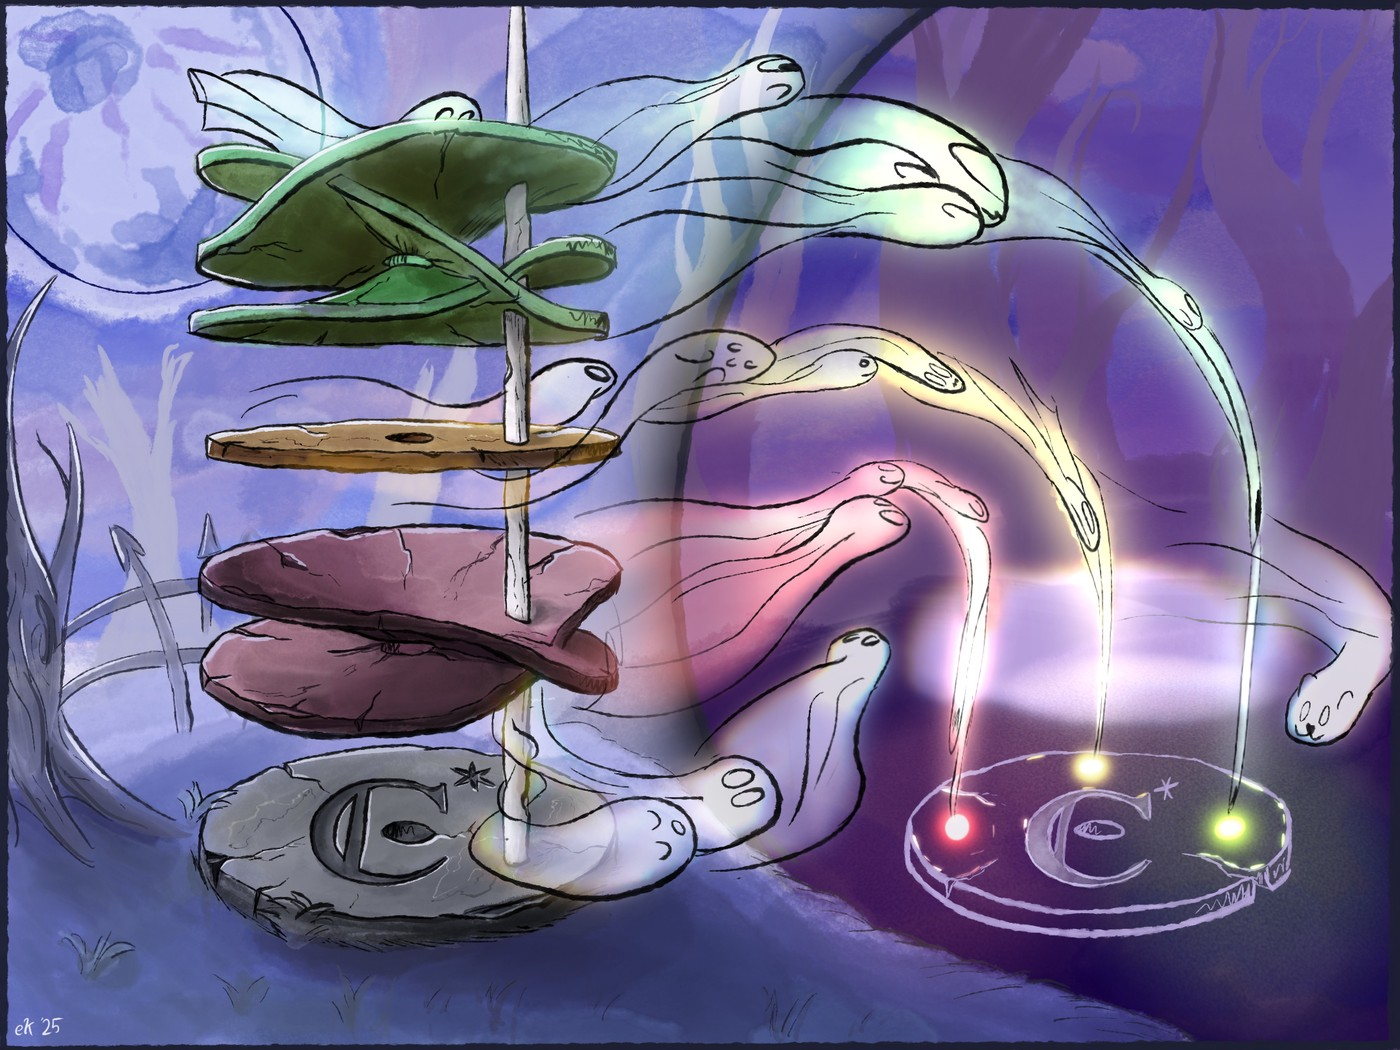
\includegraphics[width=0.74\linewidth]{figures/fig1.jpg}
\caption{层的梅林变换：谱把 $\C^{\times}_{z}$ 上的单色局部系统送到 $\C^{\times}_{t}$ 中的颜色。摩天楼对应于“白色”。（插图：Elliot Kienzle）}\label{fig:1}
\end{figure}

这些对象 $L_{t}\leftrightarrow L_{s}$ 特殊在哪里？$\C^{\times}_{z}$ 是一个群，而这些对象被称为特征层（character sheaf），因为它们的行为像这个群的特征——例如它们的解 $z^{s}$ 正好就是特征。我们可以这样表达这一想法：利用群结构，可以把局部系统沿 $w\in\C^{\times}$ 的旋转平移。$L_{t}=tz^{s}$ 是本征系统：由于 $(wz)^{s}=w^{s}z^{s}$，它们与自己的每个旋转 $w\in\C^{\times}$ 都相容地同构。对此的进一步阐发是：梅林变换把 $\Loc(\C^{\times}_{z})$ 上的卷积结构（表达 $\C^{\times}$ 的群结构）与 $\QCoh(\C^{\times}_{t})$ 上的乘法（即逐点张量积）结构等同起来。这样一来，它既是谱定理的一种形式，又是范畴化的傅里叶变换。

这契合范畴化傅里叶变换的总体主题——它们是阿贝尔群与其对偶之间各种层（导出）范畴的等价，互换卷积与张量积运算~[Lau96]。例子包括：在 $\C$、$\R$、$\F_{q}$ 上的对偶向量空间之间，分别等同 D-模、可构造层与 $\ell$-进层的 Fourier–Malgrange、Fourier–Sato 与 Fourier–Deligne 变换；以及在对偶阿贝尔簇之间等同凝聚层的 Fourier–Mukai 变换~[Muk81]。几何朗兰兹的挑战，就是为这一丰富的理论发展出非阿贝尔的对应物。

\subsection{非阿贝尔对偶的形状}\label{sec:1.4}

只要出现彼此交换的算子，傅里叶理论与谱定理的基本轮廓就适用。已知的非阿贝尔对应物则要受限得多、也精细得多。本节将勾画 Langlands 纲领与电磁 S-对偶所提供的非阿贝尔对偶的最粗略轮廓，以指出 GLC 在这两者之间所处的特殊位置。关于与物理的关系，另见 \S\ref{sec:6.2} 中略为宽广的提示。

\subsubsection{群}\label{sec:1.4.1}

我们首先固定

\begin{itemize}
\item $G$：一个约化代数群（reductive algebraic group）——例如 $\mathrm{GL}_{n}$、$\mathrm{SL}_{n}$、$\mathrm{SO}_{2n}$、$\mathrm{SO}_{2n+1}$……$E_{8}$。在 $\C$ 上（我们主要停留于此），这些正好是紧李群的复化。（我们只考虑连通群。）
\end{itemize}

每个这样的 $G$ 都伴随一个“对偶”的复\anote{更一般地，我们得到的是定义在 $G$ 的表示之定义域 $k$ 上的群——我们将假定（或假装假定）$k=\C$。}约化群，即朗兰兹对偶群（Langlands dual group）$\Gd$。关于 $\Gd$ 的总体想法是：$G$ 的各种花样的表示（即从 $G$ 出发的同态）应当对应于其对偶群中的共轭类——或更一般地，映入对偶群的同态。它可以借助李群的组合理论（根、Dynkin 图等等）具体定义：保留 $G$ 的外尔群，而把所有环面与根空间的组合结构对偶化。群 $\mathrm{GL}_{n}$ 与 $\mathrm{SO}_{2n}$ 是自对偶的；单连通群如 $\mathrm{SL}_{n}$ 与伴随群如 $\mathrm{PGL}_{n}$ 互换；奇正交群 $\mathrm{SO}_{2n+1}$ 则与辛群 $\mathrm{Sp}_{2n}$ 互换。我们将会看到，几何朗兰兹对偶给出了对偶群由何而来的根本性刻画，见 \S\ref{sec:3.3}。\zhnote{$\Gd$ 的组合定义只用到根数据（root datum）的对偶；nLab 词条 \emph{Langlands dual group} 给出了根数据对偶的完整定义与例子（$\mathrm{SL}_{n}\leftrightarrow\mathrm{PGL}_{n}$、$\mathrm{SO}_{2n+1}\leftrightarrow\mathrm{Sp}_{2n}$）：\href{https://ncatlab.org/nlab/show/Langlands+dual+group}{\texttt{https:/\allowbreak{}/\allowbreak{}ncatlab.\allowbreak{}org/\allowbreak{}nlab/\allowbreak{}show/\allowbreak{}Langlands+\allowbreak{}dual+\allowbreak{}group}}（最后修订 2014-09-07）。本译文统一作“朗兰兹对偶群”，首次出现后简称“对偶群”。}

\subsubsection{背景}\label{sec:1.4.2}

其次，我们需要选择背景。

\begin{itemize}
\item 电磁对偶涉及 4 维量子场论。对于它粗糙得多的拓扑形式（一种忽略一切动力学的“静态印记”），我们可以选任意维数不超过 4 的流形 $M$ 作为“时空”。
\item 对 Langlands 纲领，我们可以在几种“域”$F$ 中选一种：数域，如 $\Q$；局部域，如 $\R$、$\C$ 或 $\Q_{p}$；或一条（光滑射影）代数曲线 $C$ 上的有理函数域。对有限域 $\F_{q}$ 上的曲线 $C$，函数域 $F=\F_{q}(C)$ 的行为与数域非常相似。对代数闭域（如 $\F_{q}$ 或 $\C$）上的曲线 $C$，其函数域却出人意料地更像局部域。
\end{itemize}

GLC 发生在 $\C$ 上的光滑射影曲线 $C$ 上。我们同样可以把 $C$ 看作定义了一个紧黎曼面，特别是一个二维流形。因此它恰好同时嵌入这两个世界。

更一般地，两个世界之间有一种略显奇幻却极其有用的平行对应，即算术拓扑（arithmetic topology）的字典，或“纽结与素数”的类比~[Mor12]：数域与有限域上的曲线都被看作（3-流形的奇异亲戚），而局部域与代数闭域上的曲线则被看作 2-流形。

\subsubsection{对偶}\label{sec:1.4.3}

对每一组这样的输入——一个群 $G$ 与一个域 $F$ 或流形 $M$——都联系着一个对偶猜想。让我们试着在所有这些猜想中辨认出一般模式。一侧是“问题”：自守侧或 A-侧，它呈现一个与群 $G$ 及流形 $M$ 或域 $F$ 相联系的谱分解问题。这些问题以起初看来互不相干的奇异背景上的调和分析的形式出现——与数域相联系的局部对称空间 $[G]_{F}$、与代数曲线相联系的向量丛模空间 $\Bun_{G}(C)$，或 $M$ 上 Yang–Mills 方程解的模空间及其变体。值得注意的是，这些空间全都密切相关，而 GLC 正是沟通它们的桥梁，我们在 \S\ref{sec:2.2} 中讨论这一点。

另一侧是“答案”：谱侧或 B-侧。它用某个适当群（例如 $F$ 的伽罗瓦群，或 $M$ 的基本群）映入朗兰兹对偶群 $\Gd$ 的表示空间——即特征簇（character variety）$\Loc_{\Gd}$——的代数几何，来描述谱分解中可能出现的颜色。我们在 \S\ref{sec:2.3} 中讨论黎曼面／代数曲线这一 GLC 背景下的特征簇。

这些谱问题中最容易辨认的，也许要数局部 Langlands 对应（Local Langlands Correspondence, LLC）——对 $\R$ 或 $\Q_{p}$ 这样的局部域的对偶。这里自守侧由群 $G(F)$（一个实或 $p$-进李群）的所有光滑表示构成，与之相对的是关于 $\R$ 的（酉）表示的经典谱定理。LLC 试图把这些表示描述为 Langlands 参数空间 $\Loc_{\Gd}(F)$ 上的向量空间族（多重度空间），后者扮演谱定理中实直线 $\R_{t}$ 的角色。尽管 LLC 似乎不受其他背景中遇到的那些更为繁复的结构影响，过去十年间，通过把局部域视为曲线或二维流形的类比物、并引进来自 GLC 乃至最终来自物理的想法，这一领域已被彻底改变（最著名的是~[FS21]）。另见 \S\ref{sec:6.1.1}。

\subsubsection{问与答？}\label{sec:1.4.4}

把两侧标为“问题”与“答案”，传达了谱定理的心理学，也在很大程度上符合 GLC 中信息流动的方向：曲面的特征簇的几何，比模空间上层的调和分析初等得多。

然而在数域的背景下，典型的信息流向是相反的：伽罗瓦群及其表示是极其神秘而精细的对象，被用来表达数论中许多最深刻的问题，例如丢番图方程的解。把它们实现为模形式与自守形式的“颜色”，给出了算术不变量（如 $L$-函数）的一种截然不同的描述，并为来自表示论与分析的强有力工具打开了大门。

另一方面，在物理中，两侧之间的关系根本不同：量子场论中的电磁对偶是完全对称的关系，是单一理论的自同构，很像它所推广的傅里叶变换。这个自同构作用于理论的各种参数：耦合常数（交换弱耦合与强耦合）、规范群（交换 $G$ 与 $\Gd$），以及拓扑扭曲的选择——后者正是我们借以丢弃动力学、保留较粗糙拓扑信息的机制。等到我们考虑与 GLC 直接相关的拓扑场论之间的对偶时，A-侧看起来比 B-侧困难得多。然而这份来自物理的馈赠——两侧之间根本的平衡——依然处处可见，并渗透到非阿贝尔对偶的整个研究之中。\zhnote{“电磁对偶把 $G$ 换成 $\Gd$”在四维 $\mathcal{N}=4$ 超对称 Yang–Mills 中由 Montonen–Olive 对偶实现；Kapustin–Witten 进一步把它化为几何朗兰兹对偶，见 nLab 词条 \emph{S-duality} 与 \emph{Kapustin-Witten TQFT}：\href{https://ncatlab.org/nlab/show/S-duality}{\texttt{https:/\allowbreak{}/\allowbreak{}ncatlab.\allowbreak{}org/\allowbreak{}nlab/\allowbreak{}show/\allowbreak{}S-duality}}、\href{https://ncatlab.org/nlab/show/Kapustin-Witten+TQFT}{\texttt{https:/\allowbreak{}/\allowbreak{}ncatlab.\allowbreak{}org/\allowbreak{}nlab/\allowbreak{}show/\allowbreak{}Kapustin-Witten+\allowbreak{}TQFT}}（最后修订 2026-09-18）。}
